\documentclass{article}

% if you need to pass options to natbib, use, e.g.:
%     \PassOptionsToPackage{numbers, compress}{natbib}
% before loading neurips_2022

\PassOptionsToPackage{numbers}{natbib}

% ready for submission
\usepackage{code_layout}
\usepackage{header_layout}
\usepackage[final]{neurips_2022}

% to compile a preprint version, e.g., for submission to arXiv, add add the
% [preprint] option:
%     \usepackage[preprint]{neurips_2022}

% to compile a camera-ready version, add the [final] option, e.g.:
%     \usepackage[final]{neurips_2022}

% to avoid loading the natbib package, add option nonatbib:
%    \usepackage[nonatbib]{neurips_2022}

\usepackage[utf8]{inputenc} % allow utf-8 input
\usepackage[T1]{fontenc}    % use 8-bit T1 fonts
\usepackage{hyperref}       % hyperlinks
\usepackage{url}            % simple URL typesetting
\usepackage{booktabs}       % professional-quality tables
\usepackage{amsfonts}       % blackboard math symbols
\usepackage{nicefrac}       % compact symbols for 1/2, etc.
\usepackage{microtype}      % microtypography
\usepackage{xcolor}         % colors
\usepackage[xetex]{graphicx}
\usepackage{amsmath}
\usepackage{mathtools}
\usepackage[section]{placeins}
\usepackage{amssymb}% http://ctan.org/pkg/amssymb
\usepackage{pifont}% http://ctan.org/pkg/pifont
\usepackage{changepage}
\usepackage[bottom]{footmisc} % (LW) fixes clashing footnote + figures


%%%%%%%%%%%%%%%%%%%%%%%%%%%%%%%%%%%%%%%%%%%%%%%%%%%%%%%%%%%%%%%%%%%%%
\newcommand{\soptitle}{Supplementary Material}
 
\title{Learning Genome Architecture Using MSA Transformers}

% The \author macro works with any number of authors. There are two commands
% used to separate the names and addresses of multiple authors: \And and \AND.
%
% Using \And between authors leaves it to LaTeX to determine where to break the
% lines. Using \AND forces a line break at that point. So, if LaTeX puts 3 of 4
% authors names on the first line, and the last on the second line, try using
% \AND instead of \And before the third author name.
\begin{document}

\author{%
  Emaad Khwaja
  \thanks{UC Berkeley - UCSF Joint Bioengineering Graduate Program} \ \thanks{Computer Science Division, UC Berkeley, CA 94720} \\
  UC Berkeley\\
  Berkeley, CA 94702\\
  \texttt{emaad@berkeley.edu}
\And
  Lucas Waldburger \footnotemark[1] \ \thanks{Biological Systems \& Engineering Division, Lawrence Berkeley National Laboratory, CA, 94720} \\
  UC Berkeley\\
  Berkeley, CA 94702\\
  \texttt{lwaldburger@berkeley.edu}}

\maketitle
    
\begin{abstract}
Understanding genome architecture in organisms facilitates the study of gene functionality and mapping regulatory networks. Operons are a transcriptional unit that share a common regulatory mechanism and one of the most basic genome structures that are abundant in prokaryotic genomes. Traditionally, geneticists manually annotate operons by inspecting gene neighborhoods using gene-level and comparative genomic features. Existing computational methods that predict operons largely rely on gene-level features, but poorly integrate comparative genomic analysis. Recently, a deep learning model, OperonHunter, was developed that uses visual representation of genomic fragments attempts to further incorporate comparative genomic features. Since its development, transformers have gained attention for their superior performance in biological prediction tasks. Here we propose an operon MSA transformer to further improve the predictions on the operon detection task. Our hope is that a transformer can better capture genome architecture features than previous machine learning methods that detect operons.
\end{abstract}

\section{Introduction}

\subsection{Operons are transcriptional units}

Prokaryotic genomes contain gene clusters that share a common regulation mechanism in the form of an operon \cite{jacob_genetic_1961}. An operon is composed of a promoter, an operator, one or more contiguous genes in a common strand direction, and a terminator. These terms have been defined in Table \ref{table:definitions}. The genes in an operon often exhibit a similar metabolic or functional relationship and are co-transcribed on a polycistronic mRNA transcript. 
\begin{table}
\caption{Terminology used to describe common DNA sequences in an operon.}
    \label{table:definitions}
     \centering
    \begin{tabular}{lll}
            \toprule
            Term       & Definition                                                                   &  \\
            \midrule
            Promoter   & Site of transcription initiation                                             &  \\
            Operator   & Site of transcription factor binding to exhibit control over gene expression &  \\
            Gene      & Sequence that encodes the synthesis of a mRNA transcript                    &  \\
            Terminator & Site of transcription termination                                            & 
        \end{tabular}
    \bottomrule
\end{table}

One of the most widely studied operons is the \textit{lac} operon in \textit{Escherichia coli}, which controls the utilization of lactose (See Fig. \ref{fig:lac_operon}). Lactose is a disaccharide composed of galactose and glucose subunits and its catabolism is disfavored in the presence of monosaccharides that are more easily converted into energy through central metabolism. For this reason, \textit{E. coli} has evolved transcriptional control over sugar availability to maximize growth fitness in the presence of competitors. The \textit{lac} operon contains three genes involved in breaking down lactose into its respective subunits and importing lactose from the extracellular environment. When lactose is present, the gene in the \textit{lac} operon are constitutively expressed. In the presence of glucose, a transcription factor occludes the operator site thereby repressing genes in the \textit{lac} operon. Since the 1960s when the lac operon was first identified, operons have been identified across the kingdoms of life. Although they are most present in bacterial and archaeal genomes, the operon represents one of the most ubiquitous genetic structures.


\begin{figure}
  \centering
  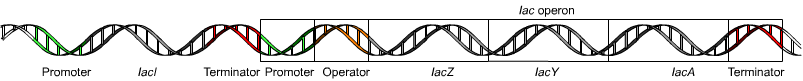
\includegraphics[width=1\textwidth]{images/lac_operon_wiki.png}
  \caption{Genetic architecture of the \textit{lac} operon required for the transport and metabolism of lactose in \textit{E. coli}. Operons share transcriptional regulation and a common promoter and terminator.}
  \label{fig:lac_operon}
\end{figure}

\subsection{Motivation}

Understanding the genome architecture in organisms facilitates the study of gene functionality and mapping regulatory networks \cite{assaf_detecting_2021}. Operon prediction represents a step toward understanding higher level gene organization and means to provide more complete gene annotations that can be applied towards identifying new antibiotics \cite{pantosti_mechanisms_2007} and anti-phage defense systems such as CRISPR-Cas9 \cite{medina-aparicio_crisprcas_2011}. Geneticists annotate operons by using gene-level information such as intergenic distance, strand direction, gene size, and functional relatedness in the same genome. In addition, a comparative genomics approach can be used to consider gene neighborhood conservation in other related genomes. Operons can be experimentally validated to further understand regulation structure. However, manual operon validation is time-consuming since genomes are large and data analysis by humans is error-prone and often subjective. For example, the genome of \textit{E. coli} consists of approximately 4,639,221 bases of DNA \cite{blattner_complete_1997}. Scattered throughout this sequence are between 630 to 700 operons \cite{salgado_operons_2000}. For this reason, there is a need for learning models that can accurately identify operons since the speed of new genomes being sequenced has rapidly outpaced the speed of functional characterization and experimental validation.

\section{Related Work}

\subsection{Existing Methods}

Existing computational methods used to predict operons largely focus on gene-level features. These methods include using Hidden Markov Models (HMMs) to identify shared promoter and terminator sequences flanking consecutive genes. Others use functional relatedness between genes in a genetic neighborhood. More advanced computational methods use machine learning to predict operons with architectures such as neural networks \cite{chen_2004,tran_2007}), support vector machines \cite{zhang_2006}, decision-tree based classification \cite{dam_2007}, Bayesian probabilities \cite{bockhorst_2003, edwards_2005, westover_2005}, genetic algorithms \cite{jacob_2005}, and graph-theoretical techniques \cite{zheng_2002,edwards_2005}. These tools have facilitated operon prediction by providing operon databases and web-based tools. However, many of tools that claim highest performance are no longer available online or have low-throughput web interfaces that limit their utility.

\subsection{OperonHunter v1.1}

A deep learning model, OperonHunter, was recently developed that uses visual representation of genomic fragments as an attempt to further incorporate comparative genomic features into operon prediction \cite{assaf_detecting_2021}. This method represents the state of the art in the operon prediction field. The authors train a visual representation learning model akin to how a geneticist would manually detect operon representations. They represented query genes as arrows with variable lengths corresponding to gene size, arrowhead directions corresponding to strand direction, arrow color corresponding to gene function class, and negative space between arrows corresponding to intergenic distance. Comparative genomic analysis is incorporated by aligning the query genes to close relatives of the query genome. The authors used a nuanced definition of an operon as containing two or more genes.

OperonHunter is trained on datasets from \textit{E. coli} and \textit{B. subtilis}, which are model prokaryotes with well-studied genomes and experimentally validated operons. The authors of OperonHunter compare their model to two existing methods claiming to have the highest accuracy. The first method, ProOPDB, uses an artificial neural network that predicts operons based on intergenic distance and gene functional relatedness \cite{taboada_high_2010}. Functional relatedness is calculated by scores in the STRING database \citet{jensen_string_2009}. The STRING database captures functional relatedness through scores using information on gene neighborhoods, fusion, co-occurrence, co-expression, protein-protein interactions, and automatic literature mining. These data are compiled into the Prokaryotic Operon Database (ProOpDB) and as a web tool called Operon Mapper. Unfortunately, ProOpDB is no longer accessible online and using Operon Mapper is extremely low-throughput which is prohibitive to large phylogenetic analyses that rely on operon predictions. The second method, Door, uses a combination of linear- (decision tree) and nonlinear-based (logistic function) classifiers depending on the availability of experimentally validated operons for the query genome \cite{mao_2014}. Door predicts operons based on intergenic distance, the presence of a DNA motif between consecutive genes, the ratio of the gene lengths and function similarity determined using Gene Ontology (GO), and the level of conservation of the genomic neighborhood.

Gene-pair prediction performance is determined by sensitivity (true positive rate), precision, and specificity (true negative rate). ProOpDB scored the highest sensitivity with the lowest precision while Door scored the lowest sensitivity and highest precision. OperonHunter performed more stably across these two metrics while scoring highest on accuracy, F1 score accuracy, and the Matthews Correlation Coefficient (MCC). On the full operon prediction task, all three tools performed substantially worse. OperonHunter had the highest performance of 85\% exact operon matches to experimentally validated genetic boundaries. Therefore, when compared to other leading methods, OperonHunter was able to achieve top performance across established datasets (See Table \ref{table:results}), with markedly better sensitivity.

% To further interrogate the inner workings of OperonHunter, Grad-Cam was used to overlay heat maps over the input images to highlight attention that most affects the model’s decisions \cite{Selvaraju_2019}. From this analysis, the authors claim that the model predicts operons using strand direction, gene neighborhood conservation through mis-alignment between genomes, and STRING score of the query gene pair which all align with important features in existing prediction methods. 

\subsubsection{Dataset}

Rather than using raw data as a source of inference, OperonHunter relies on data coming from PATRIC \cite{brettin_rasttk_2015}, a genetic visualization tool, to make predictions on whether grouped genes are in an operon. The authors of OperonHunter appear to use a completely novel procedure to produce images. In each image (see Fig. \ref{fig:operonhunterdata}), the central queried genome is placed at the top row, and related queried genes appear in the rows below. For each queried gene, a total of 5000 base pairs were pulled in the corresponding genome neighborhood, with the queried gene in the center. Each arrow represents a single gene. The authors state that each arrow is scaled to reflect it size relative to the region; however, we found this statement to be misleading.

The authors state that the image is divided into three regions, however, they fail to mention that this division is done rather arbitrarily and gene size scaling happens after this division. To clarify, the central gene (red arrow) and the one immediately following are set to a total width 50\% of the horizontal image width of 300 pixels. The regions before and after are each given 25\% of the horizontal width, and within those regions, genes are scaled accordingly. Finally, a triangular arrowhead is placed either on the left or right side of the gene depending on the transcription direction. Furthermore, at any time only a maximum of 12 genes are given unique color corresponding to gene function similarly. Any gene with a number index of 12 or higher is simply assigned a color of black. Finally, the alpha value of the operon alignment image is scaled based on a calculated STRING score from the STRING database. The STRING score is a relative measure of distance within a pre-computed graph network, which clusters proteins by similar functionality and co-incidence in literature \cite{von_mering_string_2005}.

\subsubsection{OperonHunter Architecture}

OperonHunter relies on a ResNet-18 \cite{he_deep_2015} architecture and was trained using FastAI. The authors performed data augmentation by introducing horizontal flips and zoom to images. The best performanced was trained on 50 epochs with a learning rate of 0.0001 and a batch size of 32.

\begin{figure} 
  \centering
  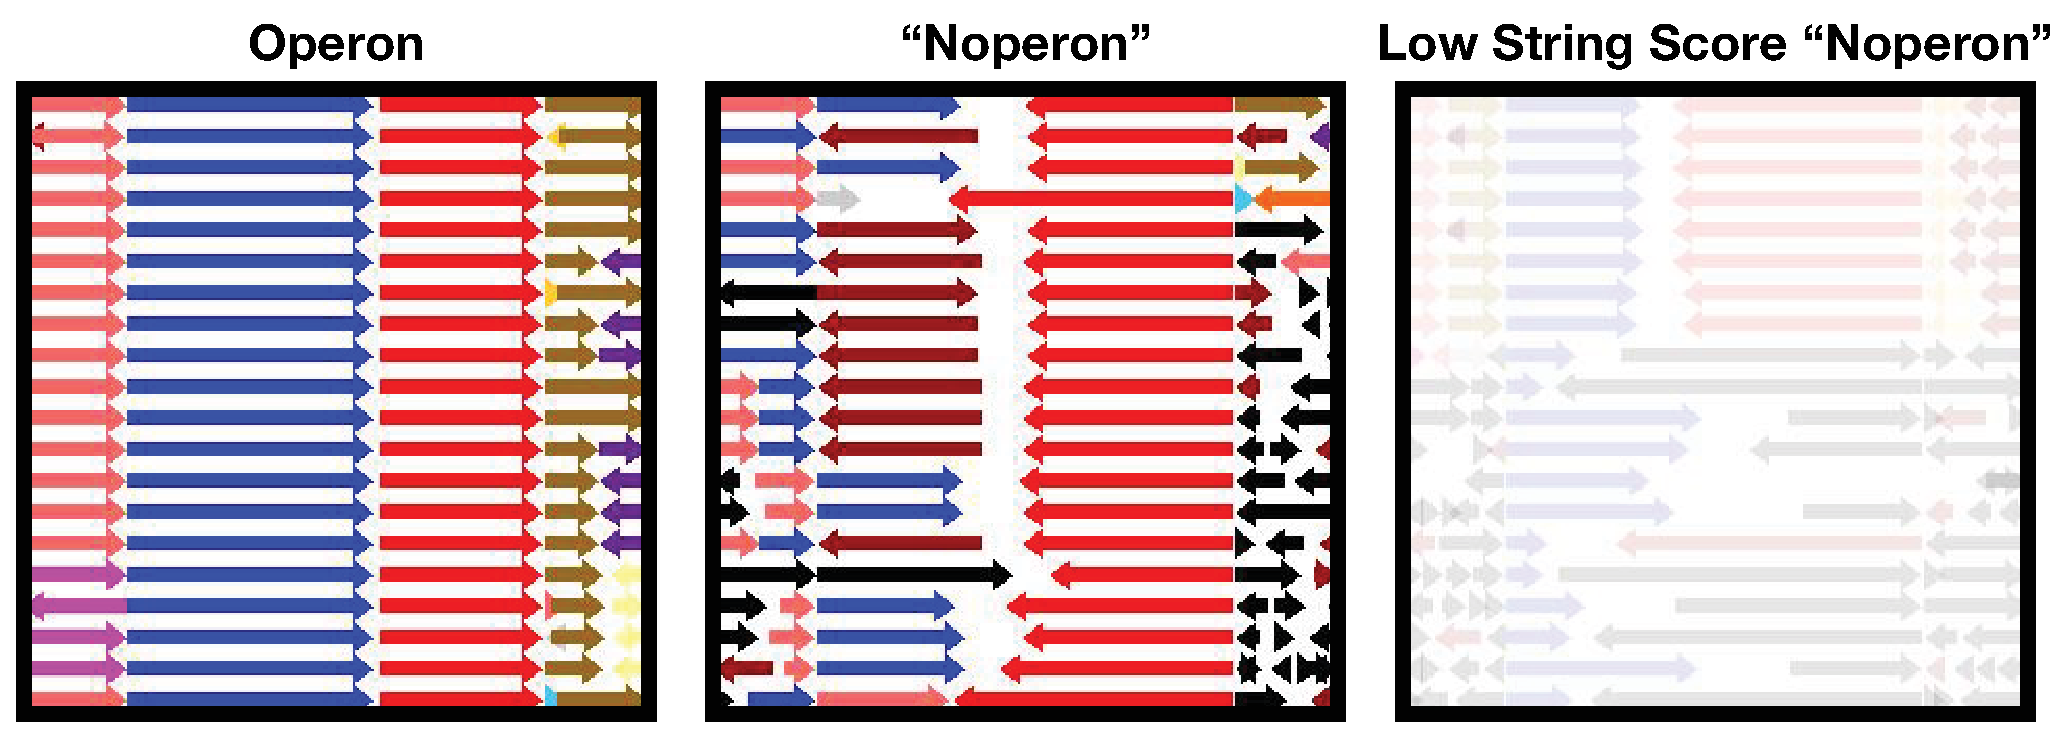
\includegraphics[width=.5\textwidth]{images/OperonHunter Image.eps}
  \caption{Operon and non-operon "noperon" images used for training. Note the incongruity in direction of arrows within the "Noperon." Low STRING scores are used to reduce the alpha channel. We noted significantly faded images such as the one displayed (right) in significantly higher frequency within the "noperon" images.}
  \label{fig:operonhunterdata}
\end{figure}

\subsubsection{Drawbacks}

Aside from the STRING score based alpha scaling, the scaling and coloring measures taken by OperonHunter merely serve to reproduce the view akin to PATRIC, however PATRIC scaling appears to be significantly different. The authors state that the generated images capture most of the prominent features mentioned earlier, such as gene conservation, functionality, strand direction, size, and intergenic distance. For the purposes of visualization, this type of data manipulation is acceptable for the sake of optimal human user experience. In the "Noperon" in Fig. \ref{fig:operonhunterdata}, we can see the procedure can result in some bizarrely truncated arrow sizing when there are many genes in the image. In the context of scientific prediction, we find the measure to be immeasurably unjustified and subject to tremendous bias.  

The authors make a point to mention the use of a pre-trained ResNet18 model, but we fail to see why this should offer any improvement. While the dataset may be small compared to ImageNet \cite{krizhevsky_imagenet_2012}, which ResNet was trained on, the operon images do not have the same level of variability in terms of image content. Furthermore, the image recognition component of a pre-trained ResNet is completely blind to the validity of an operon. If this pre-training was truly important, it would have been fairly trivial to generate an ImageNet-scale dataset by assigning random sizing, direction, and alpha values to the operon images. We believe the largest drawback of using ResNet18, or any convolutional neural network (CNN) in general, comes from the small receptive field within a convolutional kernel. Genetic function often relies on very long context. Pleitropic effectors operate on the order of thousands of base pairs. Furthermore, transcription factors may physically contort DNA sequence in 3D to bring transcriptionally distant genes in close proximity of one another \cite{vamosi_dna_2018}.

\subsubsection{Ablation}
\begin{figure} [h]
  \centering
  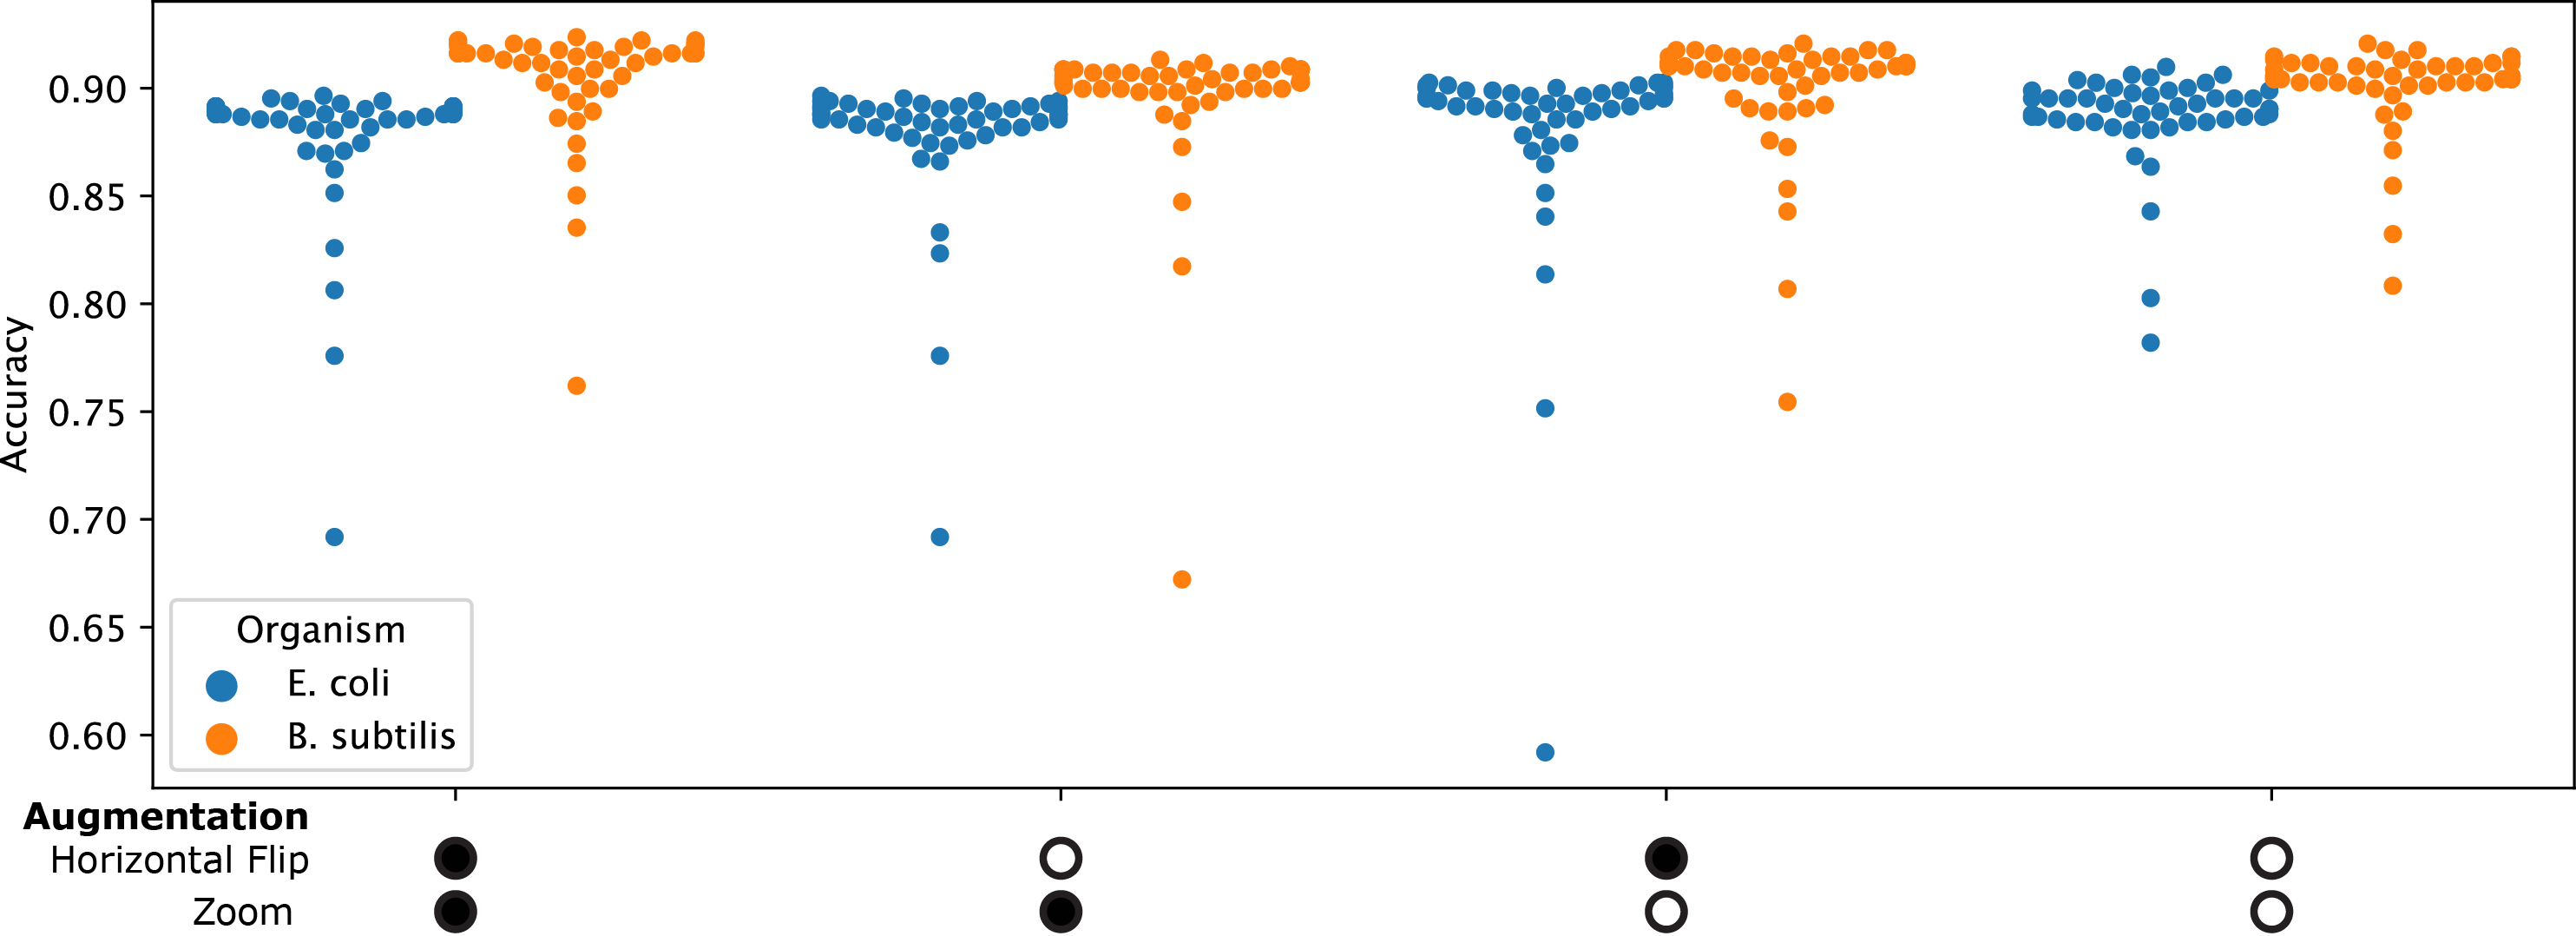
\includegraphics[width=.8\textwidth]{images/OperonHunter_ablation.png}
  \caption{OperonHunter model ablations. We tested data augmentation methods combinatorially to determine their contributions to the OperonHunter performance on the operon prediction task. The presence (solid circle) or the absence (empty circle) of a data augmentation technique.}
  \label{fig:operonhunter_ablation}
\end{figure}

We performed ablation studies on OperonHunter to interrogate the contribution to the model's performance. OperonHunter extends their dataset by performing horizontal flips and zooms on their input images. We tested the contribution of these data augmentation techniques combinatorally as shown in Fig. \ref{fig:operonhunter_ablation}. From these data, the data augmentation techniques do not significantly contribute to the predictive power of OperonHunter. A more complete ablation would include removing the alpha scaling based on STRING score in the images or removing the gene colors indicating function relatedness. However, we found the custom method of creating operon images difficult to use such that it was prohibitive to incorporate these further analyses.



\section{Methods}

We sought to demonstrate operon prediction using a machine learning model which addresses the sources of bias and architectural weaknesses of OperonHunter. We believe the introduction of sequence alignments was a truly useful source of information which could enhance Operon prediction. Specifically, the issues we sought to address were: bias and genetic under-representation or exaggeration from arbitrary scaling around the operon, extraneous data resulting from arbitrary arrow head placement and spacing between alignments, loss of long-context information from convolution, and false correlative potential coming from diagonal entries in the convolution kernel.

\subsection{Operon MSA Transformer}

We decided to implement a classifier which utilizes embeddings coming from a multiple sequence alignment (MSA) transformer \cite{rao_msa_2021}. While the original use of the MSA transformer was for protein sequence alignments, we felt the priorities of this implementation and nature of genetic transcript shared enough similarity with the intent of the MSA transformer for the architecture to be applicable. 

\subsection{Dataset}

By creating arrow-head images, \citet{assaf_detecting_2021} sought to represent both orientation and genetic locus information in an input. In order to avoid the biases created from the arbitrary image creation process, we represented the genetic alignments as 5000 \(\times\) 20 arrays (5000 base pairs \(\times\) 20 alignments per query gene). Separate channels were designated for orientation and gene index. 

Orientation values were either set to 0 for intergenic (i.e. not defined by a genetic grouping), 1 for 3' \( \rightarrow \) 5' transcription (negative direction), or 2 for 5' \( \rightarrow \) 3' transcription (positive direction). Gene ID values were assigned in a similar fashion to those in \citet{assaf_detecting_2021}. For the gene index values, we took a similar approach to the original dataset. For every alignment sample, we set the query gene index to 0. We considered a total maximum number of genes of 13, although there were alignments which contained as many as 83 unique genes within an alignment. Genes to the left of the query gene were assigned values -6 to -1, and 1 to 6 on the right side. Values were then globally incremented such that the minimum value of the array was 0. We initially tried to train directly from this input. However, we exceeded VRAM capacity on the GPU due to the fact that attention has \(O(n^{2} d)\) data complexity \cite{vaswani_attention_2017, igrinis_answer_2021}. 

We reconsidered the scaling operation performed for the original dataset, and decided it was essentially a subsampling operation. We decided to do an even sampling to remove bias. We selected every 16th base until the array was 300 bases long. Such a procedure may create interruptions and/or loss of genes, which may have been the case had we randomly sampled positions, but genes can range from 400 to 1000 bases in length. Visual inspection (See Fig. \ref{fig:subsampling}) confirmed that subsampling was likely not resulting in loss genes. However, to make sure the model was still exposed to the full set of bases, we randomly shifted the start position. For example, we may select base pairs in position \([0, 15, 31, ..., 4991]\) or \([1, 16, 32, ..., 4992]\), etc. We also introduced random horizontal flips during training.  

We implemented the transformer in Pytorch. Due to time constraints, we were only able to focus on the \textit{B. subtilis} dataset.

\begin{figure} [h]
  \centering
  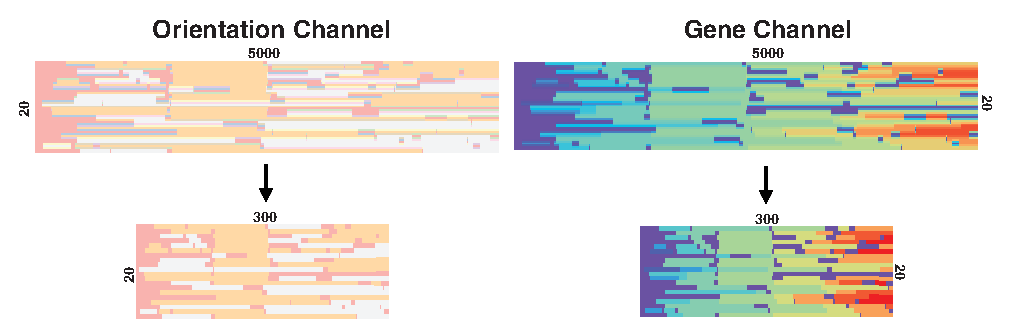
\includegraphics[width=.75\textwidth]{images/Subsampling.eps}
  \caption{Sub-sampling Procedure Depicted. Images are compressed horizontally for the sake of visualization. In the orientation channel, intergenic regions (class 0) are labelled in pink, negative orientation (class 1) is shown in white, and positive orientation (class 2) is shown in yellow. For the gene channel, each gene is given a separate color, with the intergenic regions colored in dark purple. You can see the alignment of the query gene (light green) near the center of the image. The gene color in this case is only for illustrative purposes. Integer class labels were used for training and evaluation.}
  \label{fig:subsampling}
\end{figure}

\subsubsection{Architecture}

\begin{figure} [h]
  \centering
  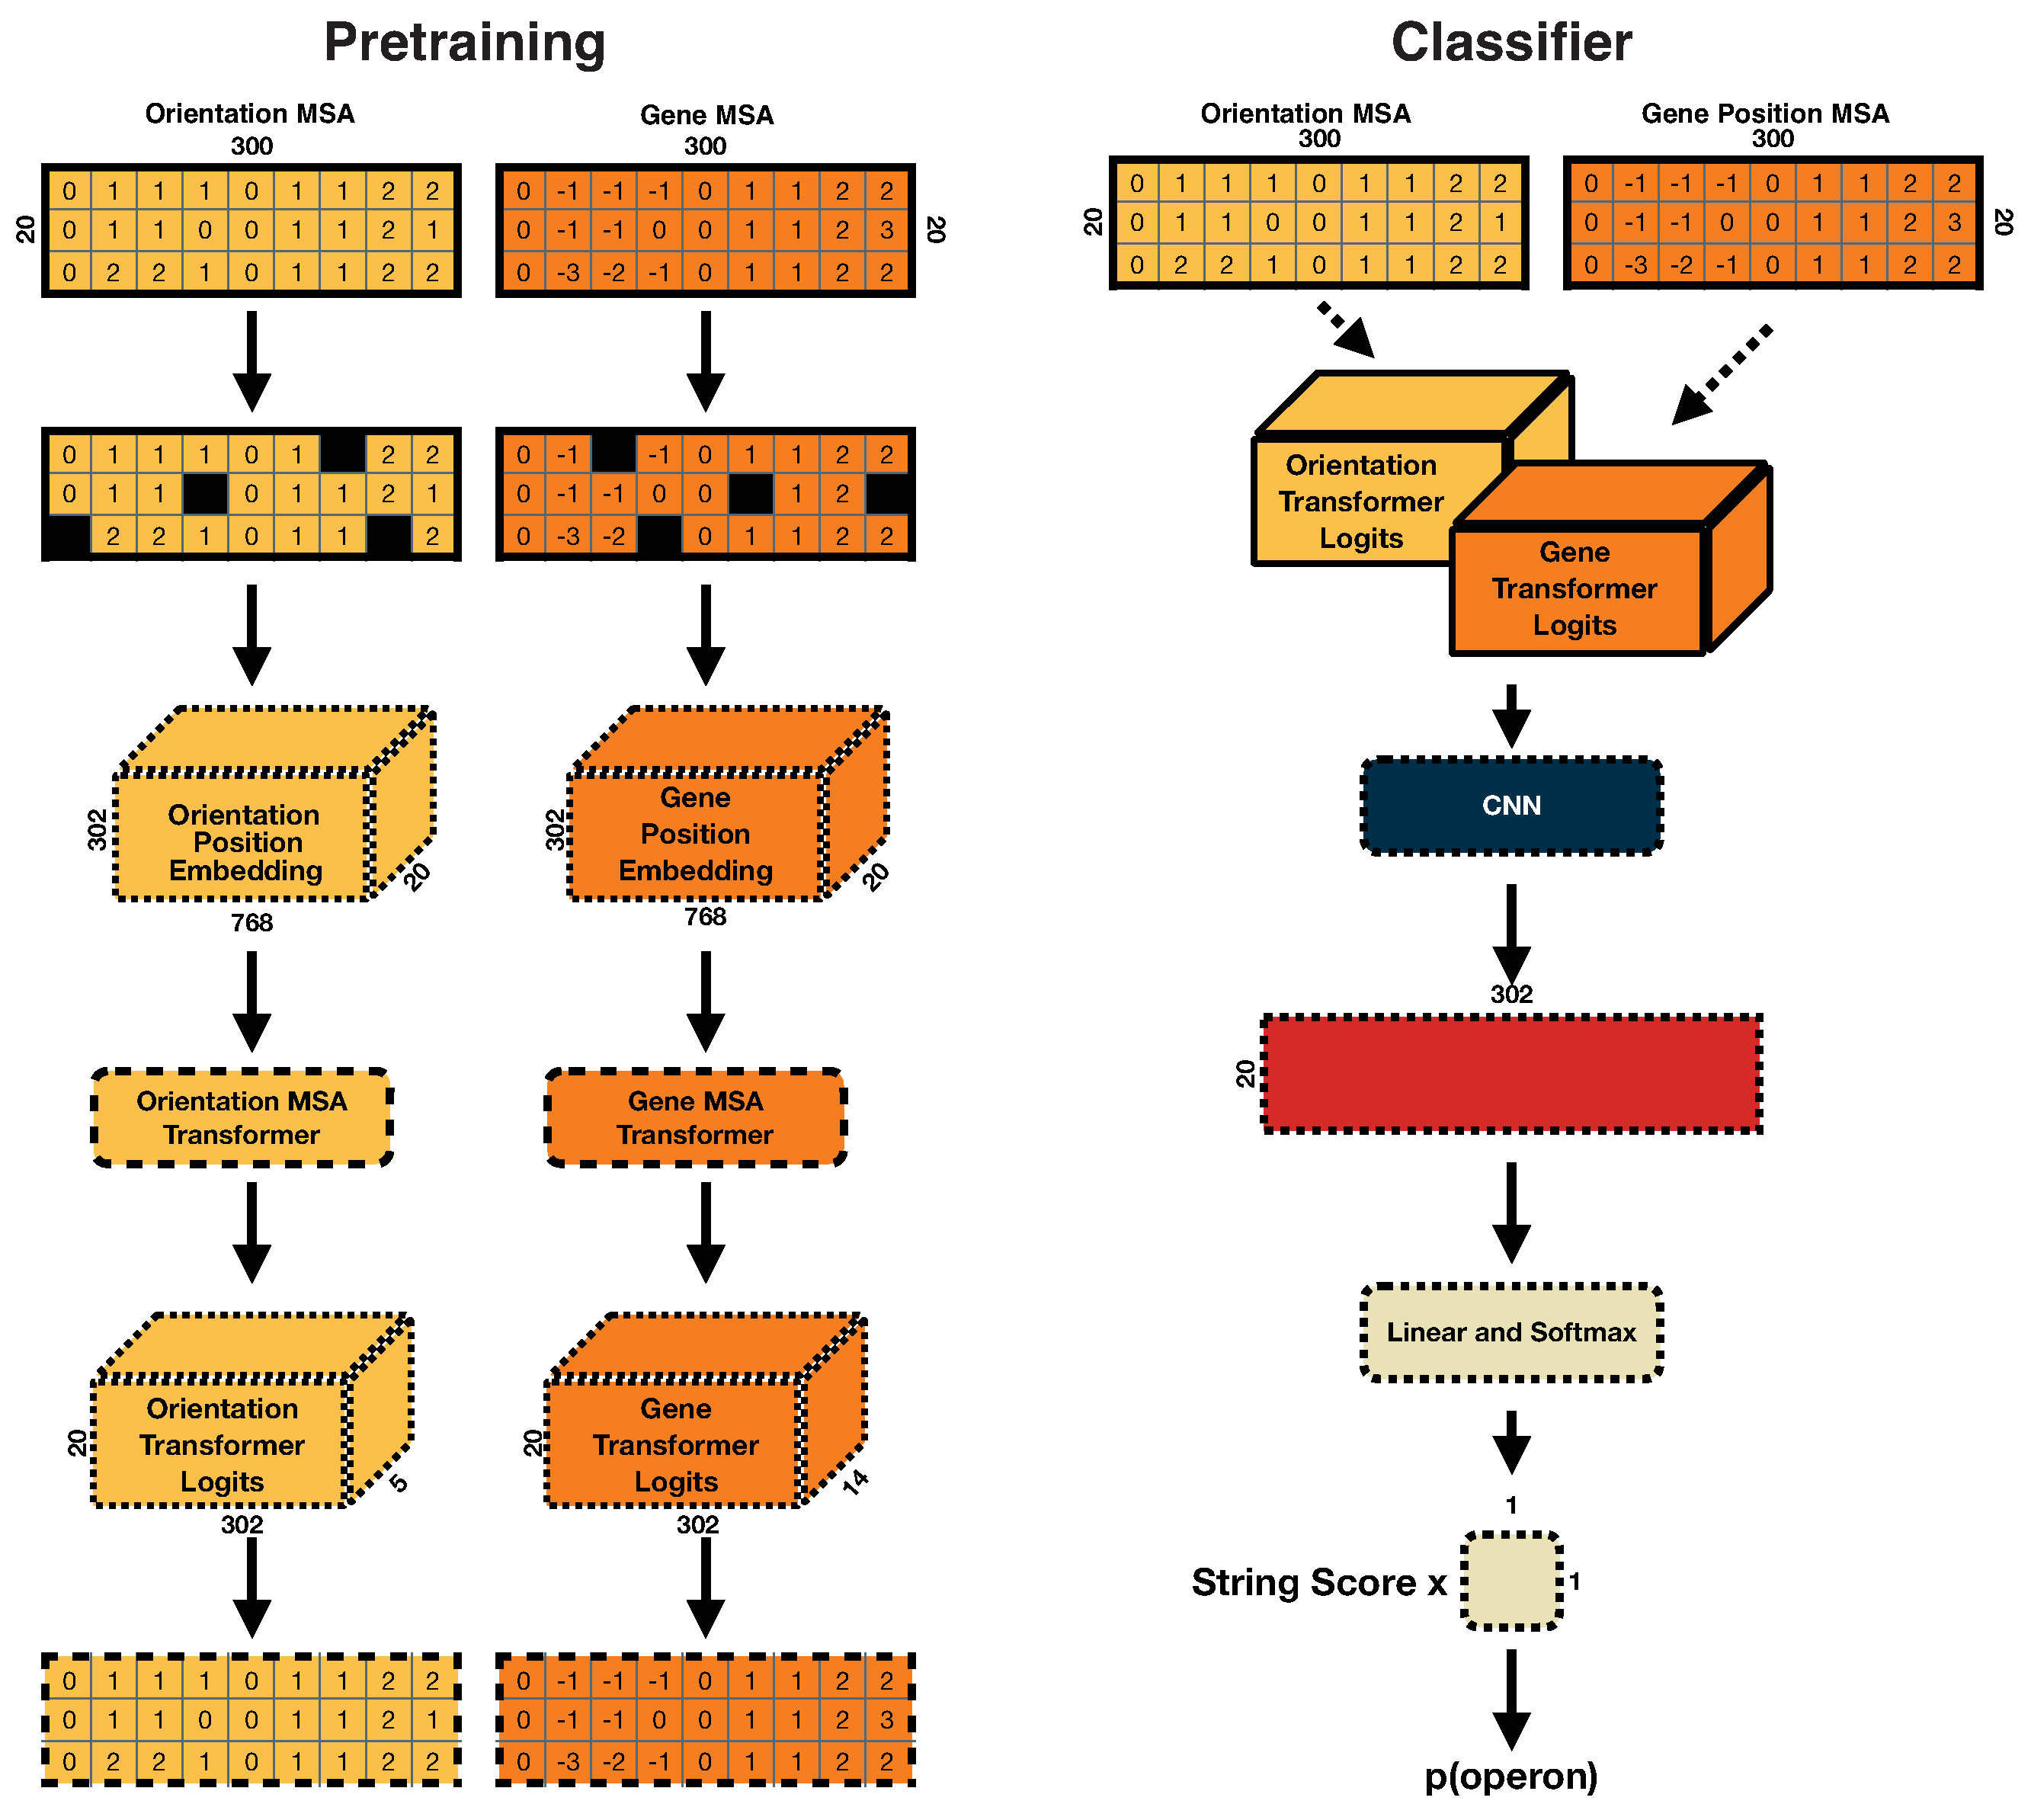
\includegraphics[width=.75\textwidth]{images/Model Diagram.eps}
  \caption{Architecture for pre-training transformer (left) which predicts masked entries, and the operon classifier (right), which outputs a probability value to predict if input is an operon. Randomly intialized values have dashed borders.}
  \label{fig:architecture}
\end{figure}

We present a visual diagram of our architecture in Fig. \ref{fig:architecture}. For the base MSA transformer,  we start with both MSA channels and apply independent random masking. We then add start and end tokens to the beginning and end of the alignments on the horizontal axis such that the tensors were of size 302 \(\times\) 20. These MSAs were then passed through a 3D embedding space of dimension 768, bringing the embedded tensors to dimension 302 \(\times\) 20 \(\times\) 768. Just as in \citet{rao_msa_2021}, we apply a learned positional embedding which is scaled based on the length and number of alignments. 

Embeddings are then passed to two separately constructed transformer modules. Each module had depth of 11, that is 11 repeating blocks of paired attention and feed forward blocks. This was the maximum number allowed by our GPU. Attention was similarly calculated using tied row and column attention.We masked the start and end token entries along the class index axis within the logits tensor by setting them to the minimum possible values, and then removed the start and end tokens along the position axis. The output logits were then converted into a predicted reconstruction of the input orientation and gene position MSAs.

The classifier utilized the output logits (with start and end tokens) from the transformer modules and stacked them along the class position axis. Zero padding was used to make the orientation logits the same size. We then used a convolutional neural network with a kernel size of 3 to collapse the logits dimension and return a 2D tensor of the same size as the original input MSA channels plus start and end tokens. This tensor was then unrolled into a 1D array and passed through a fully connected layer followed by a softmax activation function to produce a single value between 0 and 1. This value was multiplied by the STRING score to return a final value, which we designate as $p(operon)$. We utilize this value because high STRING scores have been used to classify operons with 80-90\% accuracy on their own.

For our final evaluation, we calibrated a threshold using the validation set by which any value equal to or higher would be designated as an operon.

\subsubsection{Pretraining}

We used AdamW \cite{loshchilov_decoupled_2017} as an optimizer, with learning rate set to \(.0003, \ \beta_1 = .99, \ \beta_2 = .96, \) weight decay \( = .045\) with AMSGrad. Loss was evaluated via cross-entropy. We trained over 11 epochs with a batch size of 1, with each epoch taking approximately 1.5 hours to complete.

\subsubsection{Classifier Training}

We used identical hyperparameters to the pre-training stage. The labels corresponding to each input were either 1: Operon or 0: Not Operon. Since this was a single class prediction problem, we opted to use MSE Loss rather than cross-entropy to maintain higher resolution within the weights avoid vanishing gradients.

\section{Results}

\begin{table}[h]
\caption{Model performance on the operon prediction task.}
\label{table:results}
\begin{tabular}{lcccll}
\toprule
Model              & Sensitivity (\%) & Specificity (\%) & Accuracy (\%) & MCC  & F1-Score \\
\midrule
Operon MSA Transformer & 89               & 87               & 86            & .726  & .879        \\
OperonHunter      & 97               & 88               & 92            & .84  & .921     \\
ProOpDB            & 93               & 88               & 91            & .82  & .908     \\
Door               & 86               & 97               & 89            & .908 & .886    
\end{tabular}
\bottomrule
\end{table}


After training the classifier, we evaluated on the validation set. We plot the ROC curve in Fig. \ref{fig:ROC}. From this curve, we determined the optimal cutoff threshold was .757. Output scores greater than this value were designated as operons.

\begin{figure} [h]
  \centering
  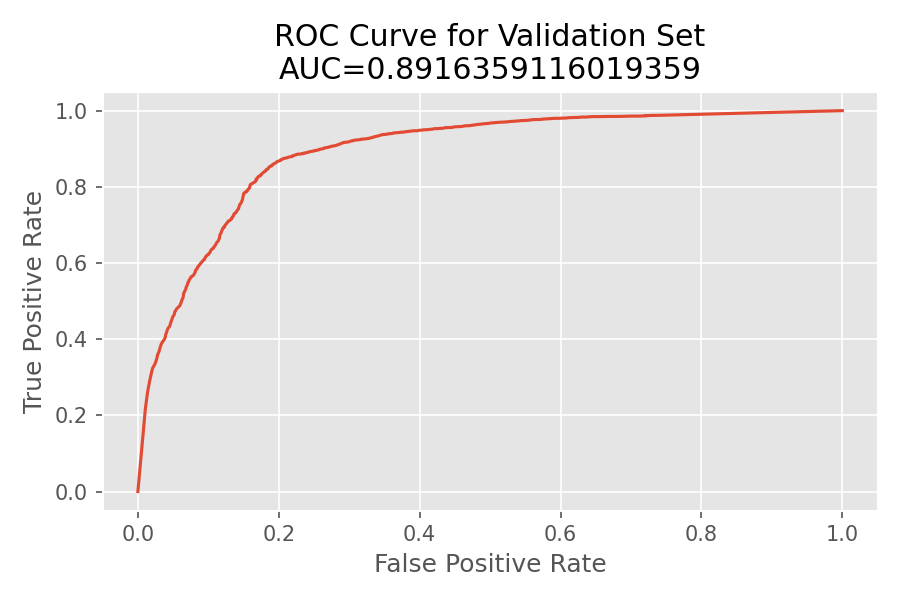
\includegraphics[width=.5\textwidth]{images/roc_curve.png}
  \caption{ROC Curve used to set cutoff threshold.}
  \label{fig:ROC}
\end{figure}

We then evaluated the performance on the test set, which we report in Table \ref{table:results}. We also report comparative values coming from \citet{assaf_detecting_2021}.


Ultimately, we were unable to outperform the reported metrics of OperonHunter using our transformer model. This may improve with extended training time or with architectural improvements, which are discussed in section \ref{discussion}.

\section{Discussion and Future Directions} \label{discussion}

OperonHunter claims effective synthesis of gene- and phylogeny-level features to predict operon by leveraging a neural network trained with image recognition capabilities. Moreover, some of the operon prediction methods include testing dataset as part of the training dataset which results in a higher accuracy as opposed to testing on novel data. The authors also fail to mention how weighing operon prediction on comparative genomic analysis limits the generalization of predictions to less well-characterized genomes. We began this project with ambitious goals which would address every single weakness of OperonHunter. While we feel our implementation significantly reduced bias, there are some considerations we would hope to address in future attempts.

% \subsection{Operon Assumptions}
 
% \citet{assaf_detecting_2021} makes an assumption in constructing the dataset that each alignment is also an operon, although we only know this to be true in the queried gene, and it is not necessarily the case that this continues to be true in the other genomes. If that assumption does not hold true, this would mean the other alignments are merely irrelevant noise rather than a source of evolutionary information.

% Furthermore, an assumption of gene identity is based solely on an ordinal relationship with the queried gene. However, it is very well possible that genes have either been mutated to become functionally different, or genes in the sequence have been completely inserted or deleted. For instance, horizontal gene transfer or transposon-mediated rearrangements can contribute to variations in genomic synteny. This actually is accounted for to some extent in the original PATRIC viewer, but which we nor \citet{assaf_detecting_2021} properly addressed.

\subsection{Additional Channels of Information}

An even subsampling of the original vector will preserve relative sizing of genes and intergenic regions so long as they are not shorter than the cut-off. The model, however is blind to absolute positional information. This may be an important factor in operon prediction as single positional insertions or deletions can result in entire frame-shift mutations, dramatically changing the operation of a genomic transcript. We initially sought to include another channel which contained indices corresponding to each horizontal position such that the model would have some information of the subsampling procedure. This, however, required a numbered class for each position (5000), which alongside having another transformer would force us to sacrifice depth of the model, which is often the most important factor in transformer performance \cite{fan_reducing_2019}. 

We also initially sought to specifically include base pairs as an additional channel. This is due to the fact that common motifs can be found in different regions, such as repeating G and C residues in non-coding portions or repeating A's in promoter sequence \cite{noauthor_frontiers_nodate}. We were ultimately unable to do so due to time and memory constraints similar to those mentioned in the previous section.

\subsection{Sampling Methods}

We opted for a regular subsampling with a random starting position, but this may not be the most representative of the dataset. We would like to explore other subsampling methods, such as random sampling. It would also be interesting to collapse the gene size by assigning indices to grouped orderings of bases, although this would come at the cost of an expanded codebook size. 

\subsection{Cross-Attention}

Our most ambitious vision involved the transformer calculating attention based on all channels simultaneously. This idea of cross attention seems to not be particularly mature, and has only been described in few recent publications. Cross-attention has so far been used as a proxy for skip exceptions in image processing models \cite{sheng_cross-attention_2022, petit_u-net_2021}, with the exception being from \citet{chang_end--end_2021}, who used recordings from three separate microphones in Amazon Echo to interpret commands. They did not release any code, and we did spend several days trying to implement, but were not able to debug in reasonable time.

\subsection{Broader Impacts}

Despite tremendous advances in targeted genome editing \cite{jinek_2012} and ambitious attempts to synthesize entire genomes \cite{richardson_2017}, there are still limited capabilities to detect some of the most basic genetic structures in prokayotic genomes. While deep learning models have proved successful in protein-related tasks such as detecting functional annotations \cite{bileschi_2022} and predicting fold \cite{jumper_2021}, the ability for such models to capture genome architecture remains elusive. 

Here we sought to extend the state of the art approach in operon prediction. We attempted to reproduce the results of OperonHunter as well as include ablation studies to interrogate the contributions of data augmentation techniques on the model's performance. We developed an operon MSA transformer to better synthesize the gene-level and comparative genomic features of operons. We view our work as a step towards understanding the design principles of genomic synteny and how this structure changes as a function of evolution.

\section*{} 
\small{
\bibliography{references.bib}
\bibliographystyle{unsrtnat}}

% \section{Code Appendix}
% \subsection{OperonHunter}
% \begin{lstlisting}[language=Python]
% print('hello world')
% \end{lstlisting}

% \subsection{Operon MSA Transformer}
% \begin{lstlisting}[language=Python]
% print('hello world')
% \end{lstlisting}

\end{document}